%
%%%%%%%%%%%%%%%%%%%%%%%%%%%%%%%%%%%%%%%%%%%%%%%%%%%%%%%%%%%%%%%%%%%%%%%%%%%%%%%%
\chapter{Theoretical background}\label{chap:1}
%%%%%%%%%%%%%%%%%%%%%%%%%%%%%%%%%%%%%%%%%%%%%%%%%%%%%%%%%%%%%%%%%%%%%%%%%%%%%%%%
%
%%%%%%%%%%%%%%%%%%%%%%%%%%%%%%%%%%%%%%%%%%%%%%%%%%%%%%%%%%%%%%%%%%%%%%%%%%%%%%%%
\section{Introduction}\label{sec:intro}
%%%%%%%%%%%%%%%%%%%%%%%%%%%%%%%%%%%%%%%%%%%%%%%%%%%%%%%%%%%%%%%%%%%%%%%%%%%%%%%%
%
Since the theoretical prediction of skyrmions in \todo{year?}
\todo{cite} and their experimental discovery in \todo{year} \todo{cite},
skyrmions have been extensively investigated both by theorists and
experimentalists \todo{some refs}. Skyrmions have caused a lot of excitement
mostly due to their promising properties that might qualify them as fast and
efficient memory. Three-dimensional non-perturbative classical Monte Carlo
methods developed recently~\cite{skyrmionlattice}, allow us to compute the full
finite temperature phase diagram and explore phase transitions. The goal of this
project was to implement a simulated annealing Monte Carlo code with the
discretized lattice Hamiltonian introduced in~\cite{skyrmionlattice} and
basically reproduce the results discussed there.  In contrast to most work on
Monte Carlo methods for spin lattices with emerging skyrmions, we want to
provide a detailed exposition of the algorithms and numerical aspects. The
report can serve as an ab initio step-by-step introduction on how to write Monte
Carlo methods and discusses associated pitfalls or caveats based on a concrete
example.  All code is publicly available on GitHub under \todo{link} and we hope
that it will be useful to others.

We introduce the model Hamiltonian in \secref{sec:model}. In
\secref{sec:mctheory} we derive Monte Carlo integration and optimization in the
framework of simulated annealing and state some important properties and results
mostly without proofs. Moreover, we discuss practical verification strategies
for Monte Carlo codes. \Secref{sec:code} contains the documentation of Sky-MoCa
as well as a quick start user manual. Finally we also provide reasoning for
design decisions. Some results and analysis of the simulations are presented in
\secref{sec:results}. However, the main goal of this paper is to illuminate the
methods more than to interpret physical results. Finally, we conclude in
\chapref{chap:3}.
%
%%%%%%%%%%%%%%%%%%%%%%%%%%%%%%%%%%%%%%%%%%%%%%%%%%%%%%%%%%%%%%%%%%%%%%%%%%%%%%%%
\section{The Spin Lattice Model}\label{sec:model}
%%%%%%%%%%%%%%%%%%%%%%%%%%%%%%%%%%%%%%%%%%%%%%%%%%%%%%%%%%%%%%%%%%%%%%%%%%%%%%%%
%
A common high-level way to think about magnetism in condensed matter is in terms
of complex collective behavior of spins, each of which is associated with a
magnetic moment. Astoundingly, this figurative model is quite powerful and
allows for a thorough explanation of a wide range of phenomena. Let us consider
a three-dimensional lattice with equidistant spacing in each direction. To each
lattice site we attach a spin, represented by an element of the unit
sphere~$S^2$, see \figref{fig:s2}. In the following we will often resort to the
two-dimensional model for illustration purposes, because it is easier to draw on
a two-dimensional surface as illustrated in \figref{fig:lattice}. However, all
computations solely concern the three-dimensional model. Each vertex of the
lattice could for example represent a nucleus in a solid with a rigid crystal
like structure. Hence the whole lattice can be interpreted as a regular atomic
structure of a solid.

\begin{figure}
  \centering
  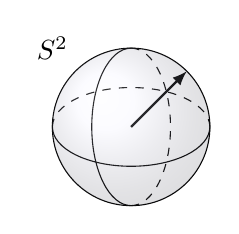
\begin{tikzpicture}
    \draw[->, thick, \select, >=latex] (0,0) -- (45:1cm);
    \draw (-1,0) arc (180:360:1cm and 0.5cm);
    \draw[dashed] (-1,0) arc (180:0:1cm and 0.5cm);
    \draw (0,1) arc (90:270:0.5cm and 1cm);
    \draw[dashed] (0,1) arc (90:-90:0.5cm and 1cm);
    \draw (0,0) circle (1cm);
    \shade[ball color=blue!10!white,opacity=0.20] (0,0) circle (1cm);
    \node at (-1,1) {$S^2$};
  \end{tikzpicture}%
  \caption{We consider three-dimensional spins, \ie{} elements of the unit
  sphere~$S^2$.}
\label{fig:s2}
\end{figure}

\begin{figure}
  \centering
  \begin{tikzpicture}
    \latticeinter{4}
    \begin{scope}[xshift=8cm,yshift=1cm]
      \lattice{4}
    \end{scope}
  \end{tikzpicture}%
  \caption{On the left side we show a two-dimensional spin lattice. Each lattice
  site carries a magnetic moment or spin, represented by an arrow of unit
  length, \ie{}, in the two-dimensional picture, by an element of~$S^1$. The
  neighbors of a lattice site are the ones above, below, left and right in the
  two-dimensional case. The blue squares are the neighbors of the red circle.
  The three-dimensional picture on the right side becomes unclear in a
  two-dimensional drawing rather quickly. Note that the magnetic moments are now
  also three-dimensional, \ie{} elements of the two-dimensional unit
  sphere~$S^2$. In three dimensions each lattice site has up to six neighbors.}
\label{fig:lattice}
\end{figure}

\todo{next to 2d and 3d lattice make drawing of only one vertex plus 6 neighbors
in 3 dimensions}

We work with a cubic lattice
%
\begin{equation}
  \Sigma := \numlist{1}{N_x} \times \numlist{1}{N_y} \times
  \numlist{1}{N_z} \subset \bN^3 \subset \bR^3\:,
\end{equation}
%
where we interpret~$(i,j,k) \in \Sigma$ as~$i \hx + j \hy + k \hz
\in \bR^3$. Here,~$\hx, \hy, \hz$ are the standard basis vectors of~$\bR^3$.
Note that we can translate the whole lattice by arbitrary integer linear
combinations of the standard basis vectors, thus starting at~$(1,1,1)$ does not
have any physical meaning. It merely corresponds nicely to the numerical
implementation in any~$1$-indexed programming language. At each point~$\r \in
\Sigma$ we attach a spin~$\S_{\r} \in S^2$, which yields the overall
configuration space~$\Pi := \prod_{\r \in \Sigma} S^2$.  Each element of~$\Pi$
consists of~$\abs{\Sigma}=N_x N_y N_z$ spins, \ie{} elements of~$S^2$, thus
describes one possible spin configuration of the whole lattice. We refer to the
specific spin at position~$\r \in \Sigma$ with~$\S_{\r} \in S^2$.  Note that
only the positions of the spins are discretized, but not explicitly their
directions. In any real implementation there is always a fine grained
discretization caused by the finite number of representable of floating point
numbers. Discrete vertices and continuous spins mirror nicely the natural
crystal structure of solids.

In a typical physical simulation one might want to find the ground state of this
system, \ie{} the lowest energy state, for some given external and internal
parameters. Necessarily, we need to define some notion of energy and also
identify some possible parameters for the spin lattice. Apparently any physical
measure of energy must be based on interactions between the spins within the
system or with external fields. Let us elaborate on some possible interactions.
Each of them comes with a constant that can be interpreted as a weight, \ie{}
how much the respective interaction contributes to the energy with respect to
the others. Let us already take away that those constants are potential
parameters of the system.

\subsection{Interactions}

\subsubsection{Ferromagnetic/direct exchange}

The most obvious interaction is the \newterm{ferromagnetic} or \newterm{direct}
exchange.  Pictorially speaking, it favors constellations where spins that are
close to each other point into the same direction. A system only interacting
this way will end up in a state where all spins are parallel to each other. The
measure for parallelism of two neighboring spins~$\S_{\r_1}, \S_{\r_2} \in S^2$
can be expressed as
%
\begin{equation}
  -\S_{\r_1} \cdot \S_{\r_2} =
  -\norm{\S_{\r_1}} \norm{\S_{\r_2}} \cos(\alpha) \:,
\end{equation}
%
where~$\alpha$ is the angle between~$\S_{\r_1}$ and~$\S_{\r_2}$. The minus sign
ensures that the energy of two parallel spins is actually smaller than the
energy of two perpendicular or even antiparallel ones.  In the continuum theory
of magnetic moments, the direct exchange term consists of a gradient, which is a
local quantity, \ie{} the gradient at a point only depends on an arbitrarily
small neighborhood of the point. Thus we will always consider the ferromagnetic
exchange to be \newterm{local} or \newterm{short ranged} in the sense that it
only contributes for adjacent lattice sites, as shown in \figref{fig:lattice}.

\subsubsection{Interaction with an external field}

Another important exchange term describes the interaction of the system with an
\newterm{external magnetic field}. Clearly, every spin tries to align with an
external field~$\B$, which we express mathematically via~$-\B \cdot \S$ for
every spin~$\S$ on the lattice. This contribution is also called the
\newterm{Zeeman energy}. It can be misleading to use terms such as
\newterm{non-local} or \newterm{long ranged} for this exchange, since it is not
an interaction between two or more spins within the system, but affects each
lattice site independently in the same way. Naturally, for the external
field,~$\B$ itself is the parameter of the interaction.

\subsubsection{Dipole-dipole interaction}

The \newterm{dipole-dipole interaction} is somewhat more complex, but also
weaker.  For two spins~$\S_{\r_1}, \S_{\r_2} \in S^2$, it is given by
%
\begin{equation}
  - {\norm{\r}^{-3}} (3 (\S_{\r_1} \cdot \hat{\r})
  (\S_{\r_2} \cdot \hat{\r}) - \S_{\r_1} \cdot \S_{\r_2})\:,
\end{equation}
%
where~$\r = \r_2 - \r_1$ and~$\hat{\r} = \r / \norm{\r}$ points from the
location of the first spin to the location of the second one. The dipole-dipole
interaction depends on the distance between the two lattice sites as well as the
orientation of the two spins not only relative to each other, but also to the
line connecting them. Moreover, the explicit dependence on the relative position
already indicates that the dipole-dipole interaction is relevant for each pair
of magnetic moments in the system, it is a long ranged interaction. In an~$N^3$
lattice, the number of pairs scales like~$N^6$. As a consequence, most
simulations do not take the dipole-dipole exchange into account purely due to
limited computational resources. We will also disregard the dipole-dipole
exchange.

\subsubsection{Dzyaloshinskii-Moriya exchange}

In this work we are interested in certain crystals that lack inversion symmetry,
\eg{} MnSi, and thus exhibit chiral magnets. The missing inversion symmetry
gives rise to the so called \newterm{weak Dzyaloshinskii-Moriya} (DM) coupling.
In the continuum it is described by a term proportional to~$-\S(\r) \cdot
(\nabla \times \S(\r))$. Just like the gradient, the curl of a vector field is a
local property, thus the DM exchange only contributes for adjacent lattice
sites. The discretized version for two spins~$\S_{\r_1}, \S_{\r_2} \in S^2$ at
neighboring positions~$\r_1, \r_2 \in \Sigma$ reads
\begin{equation}
  - (\S_{\r_1} \times \S_{\r_2}) \cdot (\r_2 - \r_1)\:.
\end{equation}
%
Since the cross product is zero for parallel vectors and maximal for
perpendicular ones, the DM coupling acts against the ferromagnetic interaction
and favors constellations where adjacent spins are perpendicular to each other.

\subsection{The Hamiltonian}

\subsubsection{Summing up the interactions}

Let us now combine the FM and DM interaction as well as an external magnetic
field to compute the energy for the lattice~$\Sigma$. To this end we add up the
contributions from each spin and for each interaction. For instance, the
external field exchange term simply becomes
%
\begin{equation}\label{Bsum}
  -\sum_{\r \in \Sigma} \S_{\r} \cdot \B\:.
\end{equation}
%

Adding up the terms for the FM interaction with all direct neighbors naively as
in
%
\begin{equation}\label{FMsumnaive}
  -\sum_{\r \in \Sigma} \S_{\r} \cdot (\S_{\r + \hx} + \S_{\r - \hx} +
    \S_{\r + \hy} + \S_{\r - \hx} + \S_{\r + \hz} + \S_{\r - \hz})\:,
\end{equation}
%
poses two problems. First, apparently in this fashion we count the interaction
between some pairs of spins multiple times. If~$\Sigma$ was an infinite grid,
\ie{}~$\Sigma=\bZ^3$, we would count every pair exactly twice and could simply
divide~\eqref{FMsumnaive} by two. However,~$\Sigma$ is finite which leads
to the second more subtle issue. Not every lattice site has a neighbor in each
direction~$\hx, \hy, \hz$. Consider the spin in the lower right corner of a
lattice in \figref{fig:lattice}. The sum in our first naive expression for the
FM interaction~\eqref{FMsumnaive} suggests that we need its right and lower
neighbor, which apparently do not exist. As a consequence, we need to define
some behavior at the boundaries. There are several ways to do this and a
plausible treatment of boundary conditions is a central aspect of many different
areas in scientific computing. It is important to realize that this is not
simply an implementation nuisance that we can get rid off by any means that make
the code work. Various boundary conditions represent different physical systems
and can significantly alter the results of a simulation.

\subsubsection{Boundary conditions}

In many cases the desired simulation volume is an infinite space, or at least so
large compared to all internal length scales that it is practically infinite. On
physical computing machines we are always limited to finite spaces. The most
obvious way for finite systems is to set all spins outside of~$\Sigma$ to zero,
\ie{}~$\S_\r = 0$ for all~$\r \in \bZ^3 \setminus \Sigma$. Consequently the
lattice sites on the boundary have less neighbors to interact with. This is
called an \newterm{open boundary}. Open boundaries are often undesirable,
because they heavily impact the behavior. In our example, a magnetic moment at
the boundary is less effected by the FM and DM interaction, simply because it
has less neighbors. However, the external field still has the same impact on a
boundary spin. This imbalance leads to polarized spins at the boundaries, \ie{}
they tend to point right in the direction of the external magnetic field~$\B$ to
maximize their Zeeman energy.

One common way to get out of this dilemma is to implement \newterm{periodic
boundary conditions}. We think of our lattice as a finite box of volume~$L^3$
for~$L\in \bRp$ and simply replicate that box infinitely many times to fill the
whole space, see \figref{fig:periodic} for a two-dimensional illustration. In
practice, we will access the lattice sites by indexing a three-dimensional array
with indices~$(i,j,k)\in\Sigma$. Whenever the algorithm tries to index out of
bounds, \eg{} requests~$j=N_y + 1$, we simply use~$j=1$ again. For~$i=0$ we
use~$i=N_x$,~$k=N_z+2$ is replaced by~$k=2$ and so on. In general, this behavior
can be achieved by always working with the indices
%
\begin{equation}\label{periodicindices}
  ((i-1 \mod N_x) + 1, (j-1 \mod N_y) + 1, (k-1 \mod N_z) + 1) \in \Sigma
\end{equation}
%
whenever the algorithm requests data at position~$(i,j,k) \in \bZ^3$. By
construction, those new indices always lie in~$\Sigma$. We can now
unproblematically include spins at officially non-existing positions in our
mathematical expressions, implicitly assuming that those are being wrapped
around periodically to positions within the lattice. This way every vertex has
the same number of neighbors.

\begin{figure}
  \centering
  \begin{tikzpicture}
    \periodic{}
  \end{tikzpicture}
  \caption{We illustrate periodic boundary conditions for a
  two-dimensional~$4\times4$ grid. The actually implemented simulation value is
  given by the shaded square in the middle. This square is copied over and over
  again in all directions as indicated by the surrounding lattice sites. Note
  how the four boundaries of the square keep their orientation throughout that
  copying procedure. While it appears like we have filled an infinite space, all
  red squares are identified, because they are represented internally by only
  one lattice site in the central square. The same holds true for the green
  pentagons of course. If our code needs the value of the right neighbor of the
  green pentagon in the central square for example, we can instead pick the
  right neighbor of \emph{any} green pentagon. One of those will always lie in
  the center square again and thus be available in memory.}
\label{fig:periodic}
\end{figure}

In our first simulations, we will employ periodic boundary conditions in all
three directions using~\eqref{periodicindices}. For other scenarios we opened up
the boundaries in one direction. This solves the second issue we encountered
in~\eqref{FMsumnaive}.

\subsubsection{Combining all interactions}

Now that we have established a well defined behavior at the boundary, we can
also tackle the first problem of counting interactions multiple times. For
periodic boundary conditions we could divide the whole expression by~$2$. In the
implementation we do not want to actually carry out redundant computations, thus
we work with
%
\begin{equation}\label{FMsum}
  -\sum_{\r \in \Sigma} \S_{\r} \cdot
    (\S_{\r + \hx} + \S_{\r + \hy} + \S_{\r + \hz})\:.
\end{equation}
%
It is worth convincing oneself that in this expression with periodic boundary
conditions every pair of neighboring lattice sites is included exactly once and
it also yields the correct results for open boundaries.

Finally, the DM term for the whole lattice is
%
\begin{equation}\label{DMsum}
  -\sum_{\r \in \Sigma} ((\S_{\r} \times \S_{\r + \hx}) \cdot \hx +
    (\S_{\r} \times \S_{\r + \hy}) \cdot \hy +
    (\S_{\r} \times \S_{\r + \hz}) \cdot \hz)\:.
\end{equation}
%
Everything we discussed about boundary conditions for the FM exchange also holds
true for the DM interaction.

Ultimately adding up all interactions~\eqref{Bsum},~\eqref{FMsum}
and~\eqref{DMsum}, we obtain the Hamiltonian, \ie{} the energy of the system in
a given configuration~$\pi \in \Pi$
%
\begin{align}\label{hamiltonian}
  H(\pi) = &-\sum_{\r \in \Sigma}\biggl(\S_{\r} \cdot \B +
      J \S_{\r} \cdot (\S_{\r+\hx} + \S_{\r+\hy} + \S_{\r+\hz}) \\
      &+ K (\S_{\r} \times \S_{\r+\hx} \cdot \hx +
            \S_{\r} \times \S_{\r+\hy} \cdot \hy +
            \S_{\r} \times \S_{\r+\hz} \cdot \hz)\biggr)\:.
\end{align}
%
The parameters~$J$,~$K$ and~$\B$ are sometimes used synonymously for the
ferromagnetic, the Dzyaloshinskii-Moriya and the external field interaction
terms. As we will see in the simulation results in \chapref{chap:3}, the
physical behavior of the system strongly depends on these freely adjustable
parameters. For a given set of parameters and at zero temperature we typically
define the physical configuration to be the
%
\begin{equation}\label{objective}
  \argmin_{\pi \in \Pi} H(\pi)\:.
\end{equation}
%

\subsubsection{Anisotropies}

% While we have remedied the problem of unwanted boundary effects due to missing
% neighbors, we are still working in a finite volume. While any real crystal also
% has a finite volume, it can typically be considered infinite relative to the
% lattice spacing. Due to computational limitations we can only simulate lattices
% with roughly~$30^3$ vertices. Thus the whole lattice is only~$30$ orders of
% magnitudes longer than the lattice spacing which leads to significant
% \newterm{finite size effects}.

In~\eqref{hamiltonian} we have collected all interactions on the lattice. Those
stem from a continuum model. Therefore we have to expect discretization errors.
In particular, the transition to a finite cubical lattice introduces
anisotropies that are absent in the original continuum model. Buhrandt and Fritz
show in~\cite{skyrmionlattice} that we can partly compensate for those
disruptive anisotropies by adding next-nearest neighbor interactions to the
Hamiltonian. The optimal choice to render higher order deviations from the
continuum model as small as possible is
%
\begin{align}\label{hamiltonianfull}
  H' := & \sum_{\r \in \Sigma} \biggl(
  \frac{J}{16} \S_{\r} \cdot (\S_{\r+2\hx} + \S_{\r+2\hy} + \S_{\r+2\hz}) \\
  &+ \frac{K}{8} (\S_{\r} \times \S_{\r+2\hx} \cdot \hx +
        \S_{\r} \times \S_{\r+2\hy} \cdot \hy +
        \S_{\r} \times \S_{\r+2\hz} \cdot \hz)\biggr)\:.
\end{align}
%
The Hamiltonian used in the simulation is then~$H + H'$. Note that~$H'$ has the
same structure of the FM and DM term of~$H$, but enters with smaller constant
and opposite sign. Adding next-nearest neighbor interactions computationally
makes a difference, but is handled the exact same way as nearest neighbor
interactions, see \figref{fig:interact}. Periodic and open boundaries still work
exactly the same way.

\begin{figure}
  \centering
  \begin{tikzpicture}
    \latticeselect{5}
    \begin{scope}[xshift=5cm]
      \latticeinter{5}
    \end{scope}
    \begin{scope}[xshift=10cm]
      \latticeinternn{5}
    \end{scope}
  \end{tikzpicture}%
  \caption{We select a spin at position~$\r \in \Sigma$ (left), show the nearest
  neighbors (middle) and the next-nearest neighbors (right). Note that although
  the diagonally neighboring vertices seem are closer to~$\r$ than the
  next-nearest neighbors, they are not included in any interaction.}
\label{fig:interact}
\end{figure}

\subsection{A note on parameter values}

Recall that there is a great conflict of interest between the FM and
the DM interactions. While the FM term in the Hamiltonian is minimal when all
spins are parallel to each other, the DM term favors a configuration where
neighboring spins are orthogonal. The specific compromise between those effects
depends mostly on their respective strength~$J$ and~$K$. In reality the direct
interaction~$J$ is much stronger and one typically encounters helical
structures with long modulation periods, see \todo{figref}. \todo{If J is
typically larger, why is here J smaller?} For example in MnSi the spins wind
around a given modulation axis only once per roughly~$40$ lattice spacings. By
tuning the ratio~$J/K$ we can set the periodicity. For a period of~$N$ lattice
sites, we have to set~$J/K$ to~$\tan(2\pi / N)$. In all our simulations we
chose~$J=1$ and~$K=\tan(2\pi / 10)$. Moreover, we let the external magnetic
field point in the~$\hz$ direction~$\B=(0,0,B)$.

We can fix one of the parameters, in this case~$J$, arbitrarily and then work in
abstract lattice units. A computer can only deal with dimensionless numbers and
in numerical simulations one often makes some convenient, but arbitrary choices.
It is then sometimes quite difficult to translate the results to physically
meaningful values.

The alert reader might have realized that so far our model does not contain any
thermal energy. When talking about magnetism, temperature typically has a strong
influence on the physical properties of various materials. However,
incorporating a temperature dependent term into the Hamiltonian that accounts
for the thermal energy is quite a challenge.  Any additive term that depends
solely on the temperature will not have any effect on~\eqref{objective}. On the
other hand there is no physical reason for complex interaction terms that
actually yield different configurations for different temperatures. Our
intuition tells us that thermal energy is intrinsically of dynamic nature, thus
cannot be captured in a single static spin configuration. In fact we will
account for temperature in the optimization algorithm itself and clearly see the
dynamic nature of it in \secref{sec:mctheory}.

\subsection{Summary}

In this section we have set up our model, which we will briefly summarize. We
work on the lattice
%
\begin{equation}
  \Sigma := \numlist{1}{N_x} \times \numlist{1}{N_y} \times
  \numlist{1}{N_z} \subset \bN^3 \subset \bR^3\:
\end{equation}
%
and attach a spin~$\S_{\r} \in S^2$ to each lattice site~$\r \in \Sigma$. This
yields the configuration space
%
\begin{equation}
  \Pi := \prod_{\r \in \Sigma} S^2\:.
\end{equation}
%
On~$\Pi$ we define the Hamiltonian~\eqref{hamiltonianfull} where we implement
periodic (and sometimes partially open) boundary conditions. We fix the
parameters~$J=1$ and~$K=\tan(2\pi / 10)$ of the FM and DM interaction, which
leaves us only with the magnetic field in the~$\hz$ direction~$B$. In the next
section we will introduce the temperature as a second parameter. Very roughly
speaking, for given values of~$B$ and~$T$ we then seek to minimize~$H(\pi)$. The
minimizing configuration is considered to be the physical one.
%
%%%%%%%%%%%%%%%%%%%%%%%%%%%%%%%%%%%%%%%%%%%%%%%%%%%%%%%%%%%%%%%%%%%%%%%%%%%%%%%%
\section{Monte Carlo Methods}\label{sec:mctheory}
%%%%%%%%%%%%%%%%%%%%%%%%%%%%%%%%%%%%%%%%%%%%%%%%%%%%%%%%%%%%%%%%%%%%%%%%%%%%%%%%
%
Now that we have clearly stated the model, let us dive into the numerics. Monte
Carlo methods stand for a broad class of numerical algorithms that are based on
some sort of repeated random sampling. The term actually stems from the casinos
in Monte Carlo, where gamblers bet on the outcome of random processes. It is
hard to formulate a more specific feature that all Monte Carlo algorithms have
in common. Most often, Monte Carlo techniques are used for optimization,
integration or sampling probability distributions. We will see soon, that
besides optimization our problem will also require us to perform
high-dimensional integrals. Before we describe our algorithm of choice in
detail, we have to issue a warning. While Monte Carlo methods are generally easy
to implement and can be applied blindly to virtually any problem, they are
almost always hopelessly inferior to specialized techniques in terms of accuracy
and efficiency. They should be the last resort after everything else has failed.
Let us start out with a general description of Monte Carlo integration and
optimization.

\subsection{Integration}

The most naive numerical integration methods like the trapezoidal rule simply
samples the integration domain by a homogeneous grid and approximates the
function by linear interpolation between the grid vertices, see
\figref{fig:int}. Of course we know how to integrate a piecewise linear function
simply by adding up the areas of the trapezoids underneath the curve.  The
important aspect here is that the choice of nodal points in the domain is
completely deterministic. Even more refined adaptive integration routines have
strict deterministic rules on how to choose their base points. In contrast,
Monte Carlo techniques sample the domain according to some probability
distribution. This is based on
%
\begin{equation}
  \int_a^b f(x) \sucd{x} = (b-a) E_{\cU[a,b]}(f)\:,
\end{equation}
%
where~$E_{\cU[a,b]}$ is simply the expectation value over the uniform
distribution~$\cU$ on the interval~$[a,b]$. This expectation value can be
approximated by averaging~$f$ over~$N \in \bN$ independent samples of~$\cU[a,b]$
%
\begin{equation}
  \int_a^b f(x) \sucd{x} \approx \frac{b-a}{N} \sum_{i=1}^N f(x_i)\:.
\end{equation}
%
Both paradigms are illustrated for a simple one-dimensional function in the top
row of~\figref{fig:int}. In this scenario the Monte Carlo integration is
absolutely not competitive. Even the crude trapezoidal rule will easily
outperform it in terms of accuracy, precision and also efficiency for a given
number of base points~$N$.

There is one more interesting aspect to Monte Carlo integration. Let us
specifically look at the integral in~\eqref{thermavgint}. The Boltzmann
factor~$\exp(-\beta H(\pi))$ assigns almost no weight to configurations with
high energy. As a consequence such configurations will not contribute much to
the overall value of the integral. This is illustrated in the second row of
\figref{fig:int}. The bulk of the area under the curve is on the left, while the
long exponential tail can practically be neglected. The trapezoidal rule, by
construction, samples the whole integration domain homogeneously, thus denotes
as much attention to the small tail as to the bulk on the left. If we were to
use Monte Carlo integration with a uniform distribution as in the top right plot
in \figref{fig:int}, many samples would fall into the right half, where the
function is basically zero. At the same time we would undersample the important
region and heavily underestimate the integral. This can be mitigated by choosing
a different probability distribution on the domain from which we draw the base
points. If we draw from an exponential distribution, almost all samples fall
within the important region and basically none are left in the insignificant
exponential tail as shown in the bottom right plot of \figref{fig:int}.

The thermal average~\eqref{thermavgint} that came up naturally in statistical
physics, like many other high-dimensional integrals encountered in physical
applications, happens to be of the form
%
\begin{equation}
  \int_{\Omega \subset \bR^n} f(x) p(x) \sucd{\lambda}_{\Omega}(x) =
  \int_{\Omega \subset \bR^n} f(x) \sucd{\mu}_{\Omega}(x)\:,
\end{equation}
%
where~$p$ is the probability density function of some measure~$\mu$ on~$\bR^n$
and~$\lambda$ is the~$n$-dimensional Lebesgue measure.

\todo{all that integration stuff needs the fact that variance is decreased when
sampling from better distribution, hence it should all be in the intro.}

\todo{guess i can leave the first section and talk about minimizing/optimizing
the energy. Later I just have to say that instead of minimizing H itself
completely on the configuration space, we minimize at certain temperature and
then average out fluctuations to get an average minimum state.}

\todo{figure out better display of axis and/or tick marks etc}
\todo{second example in figure: integrate constant function with those weights}
\begin{figure}
  \centering
  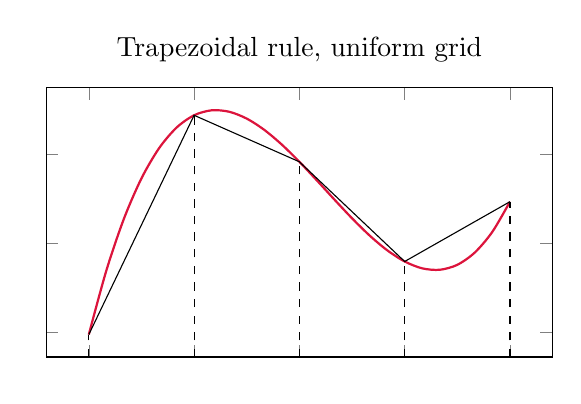
\begin{tikzpicture}[declare function={f=150 - x - 6*x^2 + x^3;}]
    \begin{axis}[
        width=8cm,
        height=5cm,
        yticklabels={,,},
        xticklabels={,,},
        domain=-2.5:5.5,
        xtick={-2.5, -0.5, ..., 5.5},
        title={Trapezoidal rule, uniform grid},
      ]
      \addplot[thick, Crimson, smooth] {f};
      \addplot[dashed, samples=5, ycomb] {f};
      \addplot[samples=5] {f};
    \end{axis}
  \end{tikzpicture}%
  \hspace{1cm}
  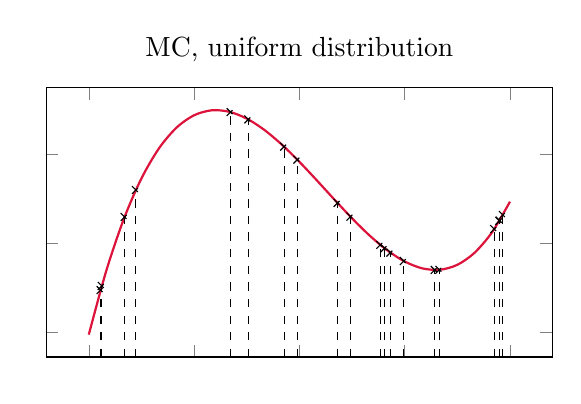
\begin{tikzpicture}[declare function={f=150 - x - 6*x^2 + x^3;}]
    \begin{axis}[
        width=8cm,
        height=5cm,
        yticklabels={,,},
        xticklabels={,,},
        domain=-2.5:5.5,
        xtick={-2.5, -0.5, ..., 5.5},
        title={MC, uniform distribution},
      ]
      \addplot[thick, Crimson, smooth] {f};
      \addplot[dashed, mark=x, samples at={3.48308, 5.29824, 1.20917,-1.60499,
      3.03779, 1.46106, 3.22893, 4.07112, 2.2248, 4.15928, 5.2014,-2.25321,
      5.30407, 0.19369,-1.81973, 2.46947,-2.27559, 3.11756, 5.36544, 0.529774},
      ycomb] {f};
    \end{axis}
  \end{tikzpicture}%
  \\
  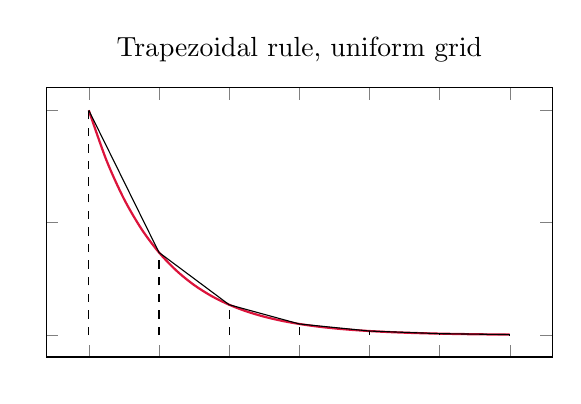
\begin{tikzpicture}[declare function={f=exp(-x);}]
    \begin{axis}[
        width=8cm,
        height=5cm,
        yticklabels={,,},
        xticklabels={,,},
        domain=0:6,
        xtick={0,...,6},
        title={Trapezoidal rule, uniform grid},
      ]
      \addplot[thick, Crimson, smooth] {f};
      \addplot[dashed, samples=7, ycomb] {f};
      \addplot[samples=7] {f};
    \end{axis}
  \end{tikzpicture}%
  \hspace{1cm}
  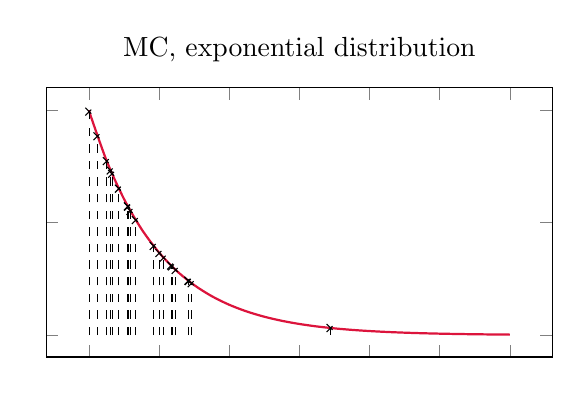
\begin{tikzpicture}[declare function={f=exp(-x);}]
    \begin{axis}[
        width=8cm,
        height=5cm,
        yticklabels={,,},
        xticklabels={,,},
        domain=0:6,
        xtick={0,...,6},
        title={MC, exponential distribution},
      ]
      \addplot[thick, Crimson, smooth] {f};
      \addplot[dashed, mark=x, samples at={1.17301, 0.559973, 0.256368, 1.00665,
      1.23844, 0.00605024, 3.44436, 0.122949, 0.311557, 0.428481, 1.06569,
      1.4651, 0.669611, 1.18508, 1.41826, 0.332201, 0.557094, 1.42344, 0.924603,
      0.593438}, ycomb] {f};
    \end{axis}
  \end{tikzpicture}%
  \caption{We show the basic principle of the trapezoidal rule in the left
  column and Monte Carlo integration in the right column. In the top row we
  consider some arbitrary function and draw from a uniform distribution in the
  Monte Carlo integration. In the bottom row we integrate the
  function~$\exp(-x)$ and sample according to an exponential distribution in the
  Monte Carlo part.}
\label{fig:int}
\end{figure}

\todo{should I actually start with integration instead of optimization for monte
carlo? --> yes!! keep optimization stuff and declare that we will need both}

\todo{the way we are sampling our space needs to contain detailed balance and
ergodicity. But why? I think that comes next and once we posed them, we
conclude that metropolis hastings might be a good idea}

\todo{replace some occurrences of ``lattice site'' by vertex}

\subsection{Optimization}

In a typical optimization problem we seek to find the minimum of a real-valued
function~$f$ over some subset of its domain~$\Omega \subset \bR^n$. Depending
on~$f$ and~$\Omega$ this can be anything from trivial to practically infeasible.
This gives rise to numerous possible classification schemes. Let us briefly
mention two important properties. First, we distinguish optimization techniques
by whether they use Hessians, gradients or only function values. Apparently the
degree of differentiability of the objective function~$f$ plays a crucial role.
If~$f$ is sufficiently smooth and we have access to gradients (and Hessians)
either analytically or numerically, we can build a first order (second order)
approximation to the function at a given point~$x \in \Omega$. This leads to so
called local methods, where we have to specify a start point, approximate the
function around this point, proceed in the downward direction and repeat the
procedure. Numerous gradient-descent and (Quasi-)Newton methods fall into that
category of iterative methods. The convergence rate and also the complexity
depend on how much information we have about the derivatives of the function,
but most iterative methods are guaranteed to converge to a minimum for
sufficiently well behaved functions and wisely chosen parameters.

The major caveat with local methods is precisely that they find \emph{a}
minimum, but potentially not \emph{the} minimum. If a function has several local
minima, depending on the start point, we might end up in any of them and
potentially overlook a global minimum somewhere else hidden to our descent
method by a barrier. In this case we could either still employ iterative methods
with multiple starting points and hope that one of them guides us to the global
minimum, or switch to heuristics. Heuristics are not mathematically guaranteed
to find the solution, in fact very little can be proven about how well
heuristics will do in general. However, they often prove very useful, especially
if we do not have an applicable finitely terminating or at least provably
convergent iterative algorithm, see \figref{fig:samplefuncs}. Interestingly,
many heuristics have been inspired by natural processes like the genetic
algorithms, bee or ant colony optimization, evolutionary algorithms or simulated
annealing.

\begin{figure}
  \centering
  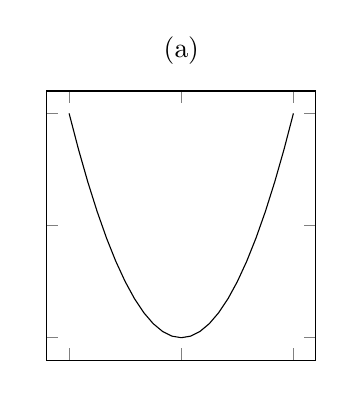
\begin{tikzpicture}
    \begin{axis}[
        width=5cm,
        height=5cm,
        title={(a)},
        % label style={font=\small},
        % xlabel={$x$},
        % ylabel={$f(x)$},
        yticklabels={,,},
        xticklabels={,,},
      ]
      \addplot[domain=-1:1] {x^2};
    \end{axis}
  \end{tikzpicture}%
  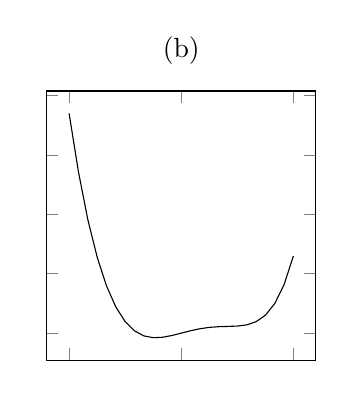
\begin{tikzpicture}
    \begin{axis}[
        width=5cm,
        height=5cm,
        title={(b)},
        % label style={font=\small},
        % xlabel={$x$},
        % ylabel={$f(x)$},
        yticklabels={,,},
        xticklabels={,,},
      ]
      \addplot[domain=-1:1] {x - 5*x^3 + 5*x^4 + 1.6*x^5};
    \end{axis}
  \end{tikzpicture}%
  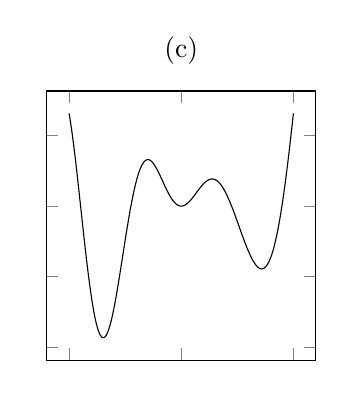
\begin{tikzpicture}
    \begin{axis}[
        width=5cm,
        height=5cm,
        title={(c)},
        % label style={font=\small},
        % xlabel={$x$},
        % ylabel={$f(x)$},
        yticklabels={,,},
        xticklabels={,,},
      ]
      \addplot[domain=-1:1, samples=1000] {sin(deg(7*x))*(x^4 - x^2 + x)};
    \end{axis}
  \end{tikzpicture}%
  \begin{tikzpicture}
    \begin{axis}[
        width=5cm,
        height=5cm,
        title={(d)},
        % label style={font=\small},
        % xlabel={$x$},
        % ylabel={$f(x)$},
        yticklabels={,,},
        xticklabels={,,},
      ]
      \addplot[solid, mark=none]
        table[x expr=\coordindex+1, y index=0] {plots/energy_landscape.csv};
    \end{axis}
  \end{tikzpicture}%
  \caption{Convex functions like the one shown in (a) can be minimized extremely
  efficiently even on high-dimensional domains. While the second example (b) is
  not convex anymore, it is smooth and has a unique minimum. Therefore local
  iterative methods will do an excellent job and converge quickly to the
  minimum. Function (c) is still smooth, but has several minima. Depending on
  where we position the starting point, iterative gradient methods might get
  stuck in one of the two local minima on the right and not find the global
  minimum on the left. The fourth function (d) is not even once differentiable
  and has numerous minima. We can only use heuristics and hope to get close to
  the true minimum.}
\label{fig:samplefuncs}
\end{figure}

The domain of our optimization problem is a~$2 N_x N_y N_z$-dimensional space.
Even for relatively small lattices optimization in such a high-dimensional space
is generically hard. Unfortunately, it appears completely hopeless to compute
the gradient or even Hessian of the Hamiltonian~\eqref{hamiltonian}
analytically. Moreover, it is hard to develop intuition about how the energy
landscape looks like, not only because we can barely visualize anything in more
than three dimensions. It appears certain, however, that it will include a vast
number of local minima. All of this is bad news for efficient iterative methods
and we have to fall back to heuristics. Our only option is to sample the search
space preferably in a smart and structured way and hope to capture the minimum
within reasonable computation time. This is precisely what Monte Carlo methods
do. They consist of a sampling strategy that involves some randomness.
Obviously, this sounds horrifically inefficient, which it is. Now we understand
why Monte Carlo techniques should only be considered once everything else failed
or proved intractable.

For our use case we implemented \newterm{simulated annealing}. The name already
hints towards thermodynamic processes, which we already identified as a key
feature of our system, but were not yet able to bake it into our model. Clearly
any real material at finite temperature is not completely static, \ie{} stuck in
a fixed state~$\pi \in \Pi$, but it is constantly subject to thermal
fluctuations. Apparently our current objective, finding a unique global minimum
of the Hamiltonian for given parameters, is insufficient. Simulated annealing is
designed to mimic real world systems at finite temperature and will take care of
thermal fluctuations. That implies that we will not seek to find a single best
state~$\pi \in \Pi$ anymore, but consider the physical state to be a thermal
average of several configurations. To fully understand and appreciate simulated
annealing, we need some basic concepts from statistical physics.

In macroscopic complex many body systems such as gases or condensed matter at
finite temperature, we are often not interested in every single detail of that
system at a given moment in time.  For example, we do not want to know the
position and velocity as well as rotational and vibrational modes of each single
molecule in a piston. Sensible observables are typically some sort of
macroscopic averages like the volume, temperature or pressure of the gas. For a
solid we might be interested in its specific heat, conductivity or
susceptibility. Of course, there is a sound and rigorous way to define those
averages.

Instead of working with the complete microstates, in our case the elements
of~$\Pi$, directly, we only talk about the probability~$P_{T}(\pi)$ that the
system is in a certain state~$\pi \in \Pi$ at temperature~$T$. To this end we
imagine a large ensemble of exact replicas of the system and observe them all at
the same time figuratively counting how often each microstate occurs. Starting
from the assumption that in a closed system in equilibrium each microstate~$\pi$
is equally likely, we can derive the so called canonical ensemble which states
that for a non-closed system in equilibrium at finite temperature~$T$, \eg{} via
contact to a large heat bath, the probability of state~$\pi$ is
%
\begin{equation}\label{boltzmann}
  P_{T}(\pi) = \frac{\exp \left(- \frac{H(\pi)}{k_B T}\right)}
  {\sum_{\pi \in \Pi} \exp \left(- \frac{H(\pi)}{k_B T}\right)}\:.
\end{equation}
%
This is also referred to as the \newterm{equilibrium Boltzmann distribution}
with~$k_B$ being the Boltzmann constant. For a finite configuration space these
are discrete probabilities that add up to one by construction.  The normalizing
factor in~\eqref{boltzmann}~$Z := \sum_{\pi \in \Pi} \exp(-\beta H(\pi))$ is
called partition function. Here we introduced the common shortcut~$\beta :=
{(k_B T)}^{-1}$. In our case there are infinitely many states in~$\Pi$ and the
summation in the partition function turns into an integral~$Z := \int_{\Pi}
\exp(-\beta H(\pi)) \sucd{\mu}_{\Pi}(\pi)$, where the measure~$\mu_{\Pi}$
depends on the configuration space. The mathematical details are not important
for the further treatment here.

The equilibrium Boltzmann distribution~\eqref{boltzmann} tells us that
configurations with lower energy are exponentially more likely than
configurations with higher energy. Moreover, this effect is most pronounced at
low temperatures. If~$T$ is large, states with higher energy still occur with a
decent probability compared to the minimizing state. On the other hand, for~$T
\to 0$, basically only the state with minimal energy has a non-zero probability.
Both facts match our intuition. At high temperatures, thermal fluctuations are
large and the system can visit many different micro states. At zero temperature
we expect the system to settle in the ground state.

In a probabilistic description of states, the energy or magnetization of one
single specific configuration looses its significance. Instead we measure
expectations values of observables. For an observable~$\map{\cO}{\Pi}{\bR}$ we
compute the so called \newterm{thermal average}
%
\begin{equation}\label{thermavgsum}
  \avg{\cO} := \frac{1}{Z} \sum_{\pi \in \Pi} \cO(\pi) \exp(- \beta H(\pi))\:,
\end{equation}
%
hence we average over all states weighted by their probability at a given
temperature. Again for a continuous state space this becomes
%
\begin{equation}\label{thermavgint}
  \avg{\cO} := \frac{1}{Z} \int_{\Pi} \cO(\pi) \exp(- \beta H(\pi))
    \sucd{\mu}_{\Pi}(\pi)\:.
\end{equation}
%

In our case the observables we are primarily interested in are the
energy~$\avg{H}$ and the three components of the magnetization~$\avg{\M} =
\avg{\sum_{\r \in \Sigma} \S_{\r}}$. One question immediately poses itself: How
could be possibly compute the high-dimensional integral in~\eqref{thermavgint}
for our specific situation? Even for finite configuration spaces the sum
in~\eqref{thermavgsum} would contain extraordinarily many terms. If each lattice
site could only be in two states, up or down, already on a small~$10^3$ lattice
we would have to sum up~$2^{1000} \approx 10^{300}$ configurations. This is far
beyond the possibilities of any machine imaginable today. The large
dimensionality of the problem renders it a good fit for Monte Carlo methods.
